% Diapositiva 04
%Danilo
%===========================================
%   2. Qué es una fuente sísmica.
%===========================================



\begin{frame}{Modelo Geométrico de la Fuente Sísmica}
    \begin{figure}
        \centering
   
        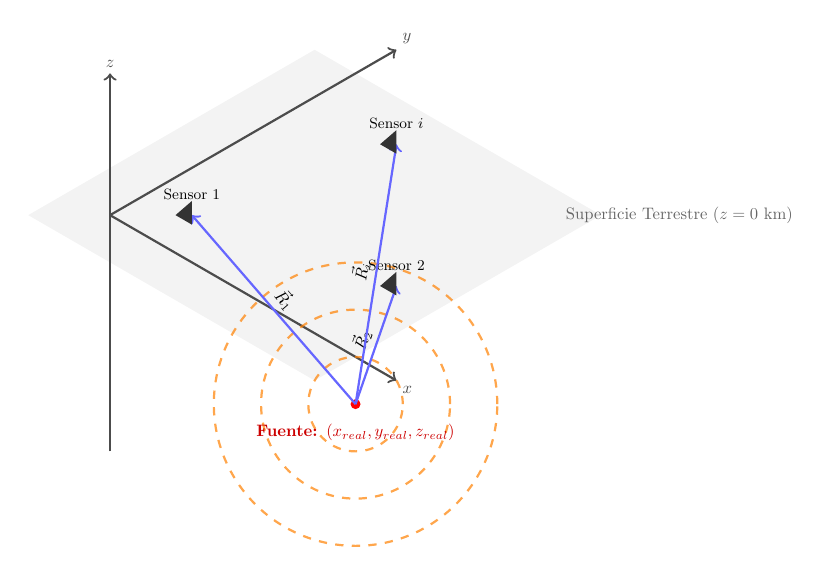
\begin{tikzpicture}[x={(0.866cm,-0.5cm)}, y={(0.866cm,0.5cm)}, z={(0cm,1cm)}, scale=0.6, transform shape]
            
            % 1. Plano de la superficie terrestre (z = 0)
            \fill[gray!10, opacity=0.9] (-1,-1,0) -- (6,-1,0) -- (6,6,0) -- (-1,6,0) -- cycle;
            \draw[gray!40, thin, step=1] (-1,-1,0) grid (6,6,0);
            \node[anchor=west, text=gray!80!black] at (5.5, 5.5, 0) {Superficie Terrestre ($z=0$ km)};

            % 2. Ejes Coordenados
            \draw[thick,->, black!70] (0,0,0) -- (7,0,0) node[below right] {$x$};
            \draw[thick,->, black!70] (0,0,0) -- (0,7,0) node[above right] {$y$};
            \draw[thick,->, black!70] (0,0,-5) -- (0,0,3) node[above] {$z$};

            % 3. Fuente Sísmica (Hipocentro)
            \coordinate (Hipocentro) at (3, 3, -4);
            
            % Frentes de onda (representados como círculos concéntricos punteados)
            \foreach \r in {1, 2, 3} {
                \draw[orange, thick, dashed, opacity=0.7] (Hipocentro) circle (\r cm);
            }
            
            % Punto central de la fuente
            \fill[red] (Hipocentro) circle (3pt);
            \node[below, font=\bfseries, text=red!80!black, yshift=-3mm] at (Hipocentro) {Fuente: $(x_{\text{real}}, y_{\text{real}}, z_{\text{real}})$};

            % 4. Sensores en la superficie y vectores de distancia
            % Coordenadas de los sensores
            \coordinate (S1) at (1, 1, 0);
            \coordinate (S2) at (5, 2, 0);
            \coordinate (S3) at (2, 5, 0);

            % Bucle para dibujar cada sensor y su vector R
            \foreach \pos/\name in {S1/1, S2/2, S3/i} {
                % Dibujar el vector de distancia R primero para que quede debajo del sensor
                \draw[->, thick, blue!60] (Hipocentro) -- (\pos) node[midway, sloped, above, text=black] {$\vec{R}_{\name}$};
                
                % Dibujar el sensor (un pequeño triángulo/pirámide)
                \fill[black!80] (\pos) + (0,0,0.3) -- + (-0.2,-0.2,0) -- + (0.2,-0.2,0) -- cycle; 
                \node[above, font=\small, yshift=2mm] at (\pos) {Sensor $\name$};
            }

        \end{tikzpicture}
        % En las presentaciones, las descripciones cortas funcionan mejor
        \caption{Propagación de ondas y vectores de distancia en $\mathbb{R}^{3}$.}
        \label{fig:fuente_3d}
    \end{figure}
\end{frame}